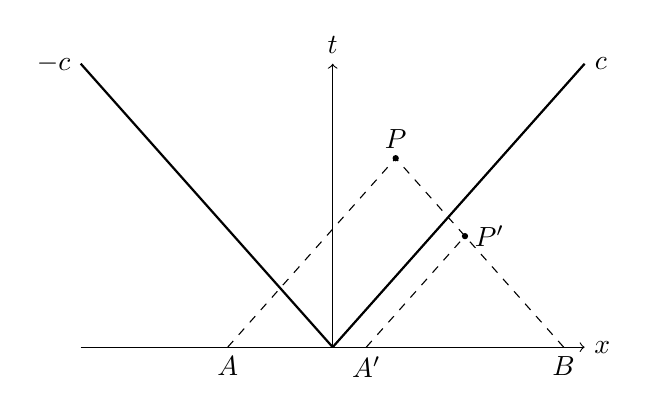
\begin{tikzpicture}[scale=0.8]
  \draw[->] (-4,0) -- (4.,0) node[right] {$x$};
  \draw[->] (0,0) -- (0,4.5) node[above] {$t$};
  \draw[thick] (0,0) -- (4.,4.5) node [right] {$c$};
  \draw[thick] (0,0) -- (-4.,4.5) node [left] {$-c$};
  \fill[black] (1.,3.) circle (0.05) node [above] {$P$};
  \draw[dashed] (1-8./3.,0.) node [below] {$A$}  -- (1.,3.);
  \draw[dashed] (1+8./3.,0.)node [below] {$B$}  -- (1.,3.);
  %% Intersection of positive solid line and negative dashed one
  %\fill[black] (0.5+12/9.,2.) circle (0.05) node [above] {$P'$};
  \fill[black] (2.10,1.762499) circle (0.05) node [right] {$P'$};
  \draw[dashed] (0.5333,0.) node [below] {$A'$}  -- (2.10,1.762499);
\end{tikzpicture}



%%% Local Variables:
%%% mode: latex
%%% TeX-master: "../../mainManuscript"
%%% End:
